\documentclass[12pt]{article}

% ========== Paquetes ===========

% Codificación de caracteres e idioma
\usepackage[utf8]{inputenc}
\usepackage[spanish]{babel}

% Paquete para referencias bibliográficas
\usepackage[backend=biber]{biblatex}

% Tamaño de página y márgenes
\usepackage[letterpaper, margin=2.54cm]{geometry}

% Comillas, columnas, gráficos, símbolos matemáticos e ingreso de código de programación
\usepackage{csquotes, multicol, graphicx, amssymb, amsmath, listings, xcolor}

% Tablas más potenciadas
\usepackage{array}

% Para hacer mosaico de figuras
\usepackage{subcaption}

% Links en texto
\usepackage{hyperref}

% Interlineado 1.5
\usepackage{setspace}
\onehalfspacing

% Color para código SQL, SQLite
\definecolor{codegreen}{rgb}{0,0.6,0}
\definecolor{codegray}{rgb}{0.5,0.5,0.5}
\definecolor{codepurple}{rgb}{0.58,0,0.82}
\definecolor{backcolour}{rgb}{0.95,0.95,0.92}
\lstdefinestyle{mystyle}{
    backgroundcolor=\color{backcolour},   
    commentstyle=\color{codegreen},
    keywordstyle=\color{magenta},
    numberstyle=\tiny\color{codegray},
    stringstyle=\color{codepurple},
    basicstyle=\ttfamily\footnotesize,
    breakatwhitespace=false,         
    breaklines=true,                 
    captionpos=b,                    
    keepspaces=true,                 
    numbers=left,                    
    numbersep=5pt,                  
    showspaces=false,                
    showstringspaces=false,
    showtabs=false,                  
    tabsize=2
}
\lstset{style=mystyle}

% \usepackage{uarial}
% \renewcommand{\familydefault}{\sfdefault}

% Uso de punto decimal, en lugar de coma
\decimalpoint

% Separación de columnas y sangría
\setlength{\columnsep}{2cm} 
\setlength{\parindent}{0cm}

% Páginado
\pagestyle{plain}

% Evitar separación de palabras
\hyphenpenalty=10000
\exhyphenpenalty=10000
\sloppy

% Archivo de referencias bibliográficas
\addbibresource{bib/referencias.bib}

% ========== Documento ==========

\begin{document}

% ========== Portada ============
\begin{titlepage}
	\centering
	{\scshape\LARGE Universidad Aztlán \par}
	\vspace{1cm}
	{\scshape\Large Campus Playa del Carmen \par}
	\vspace{1.75cm}
	{\scshape\Huge Base de Datos de un bachillerato técnico para gestión del nuevo ingreso \par}
    \vfill
    {\itshape\Large Fundamentos de bases de datos \par}
	\vspace{2cm}
    {\itshape\Large Presentado por: \par}
	{\Large José Rosendo Camal Teh \par}
	\vfill
	{\Large Ingeniería en Sistemas Computacionales \par}
	{\Large Cuarto Cuatrimestre \par}
	{\Large Fundamentos de Bases de Datos \par}
	\vfill
	{\Large Mtro. Irvin Arlin Chan Ac \par}
	\vfill
	{\Large 25 de septiembre de 2026 \par}
	\vfill
	{\Large Playa del Carmen, Quintana Roo \par}
\end{titlepage}
\newpage

\tableofcontents
\newpage

% ========== Cuerpo =============


% Investiga una base de datos relacional que hayas trabajado anteriormente en algún proyecto, ya sea un proyecto escolar de alguna otra asignatura o un proyecto de trabajo, si no haz desarrollado alguna, investiga en algún libro o en internet. Realiza una breve descripción de qué trata la base de datos y qué tipo de información almacena.
\section*{\centering Gestión del nuevo ingreso de una institución académica}
\addcontentsline{toc}{section}{Gestión del nuevo ingreso de una institución académica}

Una institución de bachillerato técnico en cada ciclo escolar gestiona el nuevo ingreso seleccionando los aspirantes y vinculando al estudiante a un plantel y una carrera técnica. El alcance del registro corresponde a un nivel estatal y para ello, se hace uso de una base de datos~\cite{rosendocamal} implementada según las necesidades mediante el SGBD de \textbf{SQLite}. Esta base de datos permite almacenar los vínculos entre aspirantes y la carrera al que fue asignada, los planteles y la oferta académica de cada plantel.

\begin{figure}[htb]
	\centering
	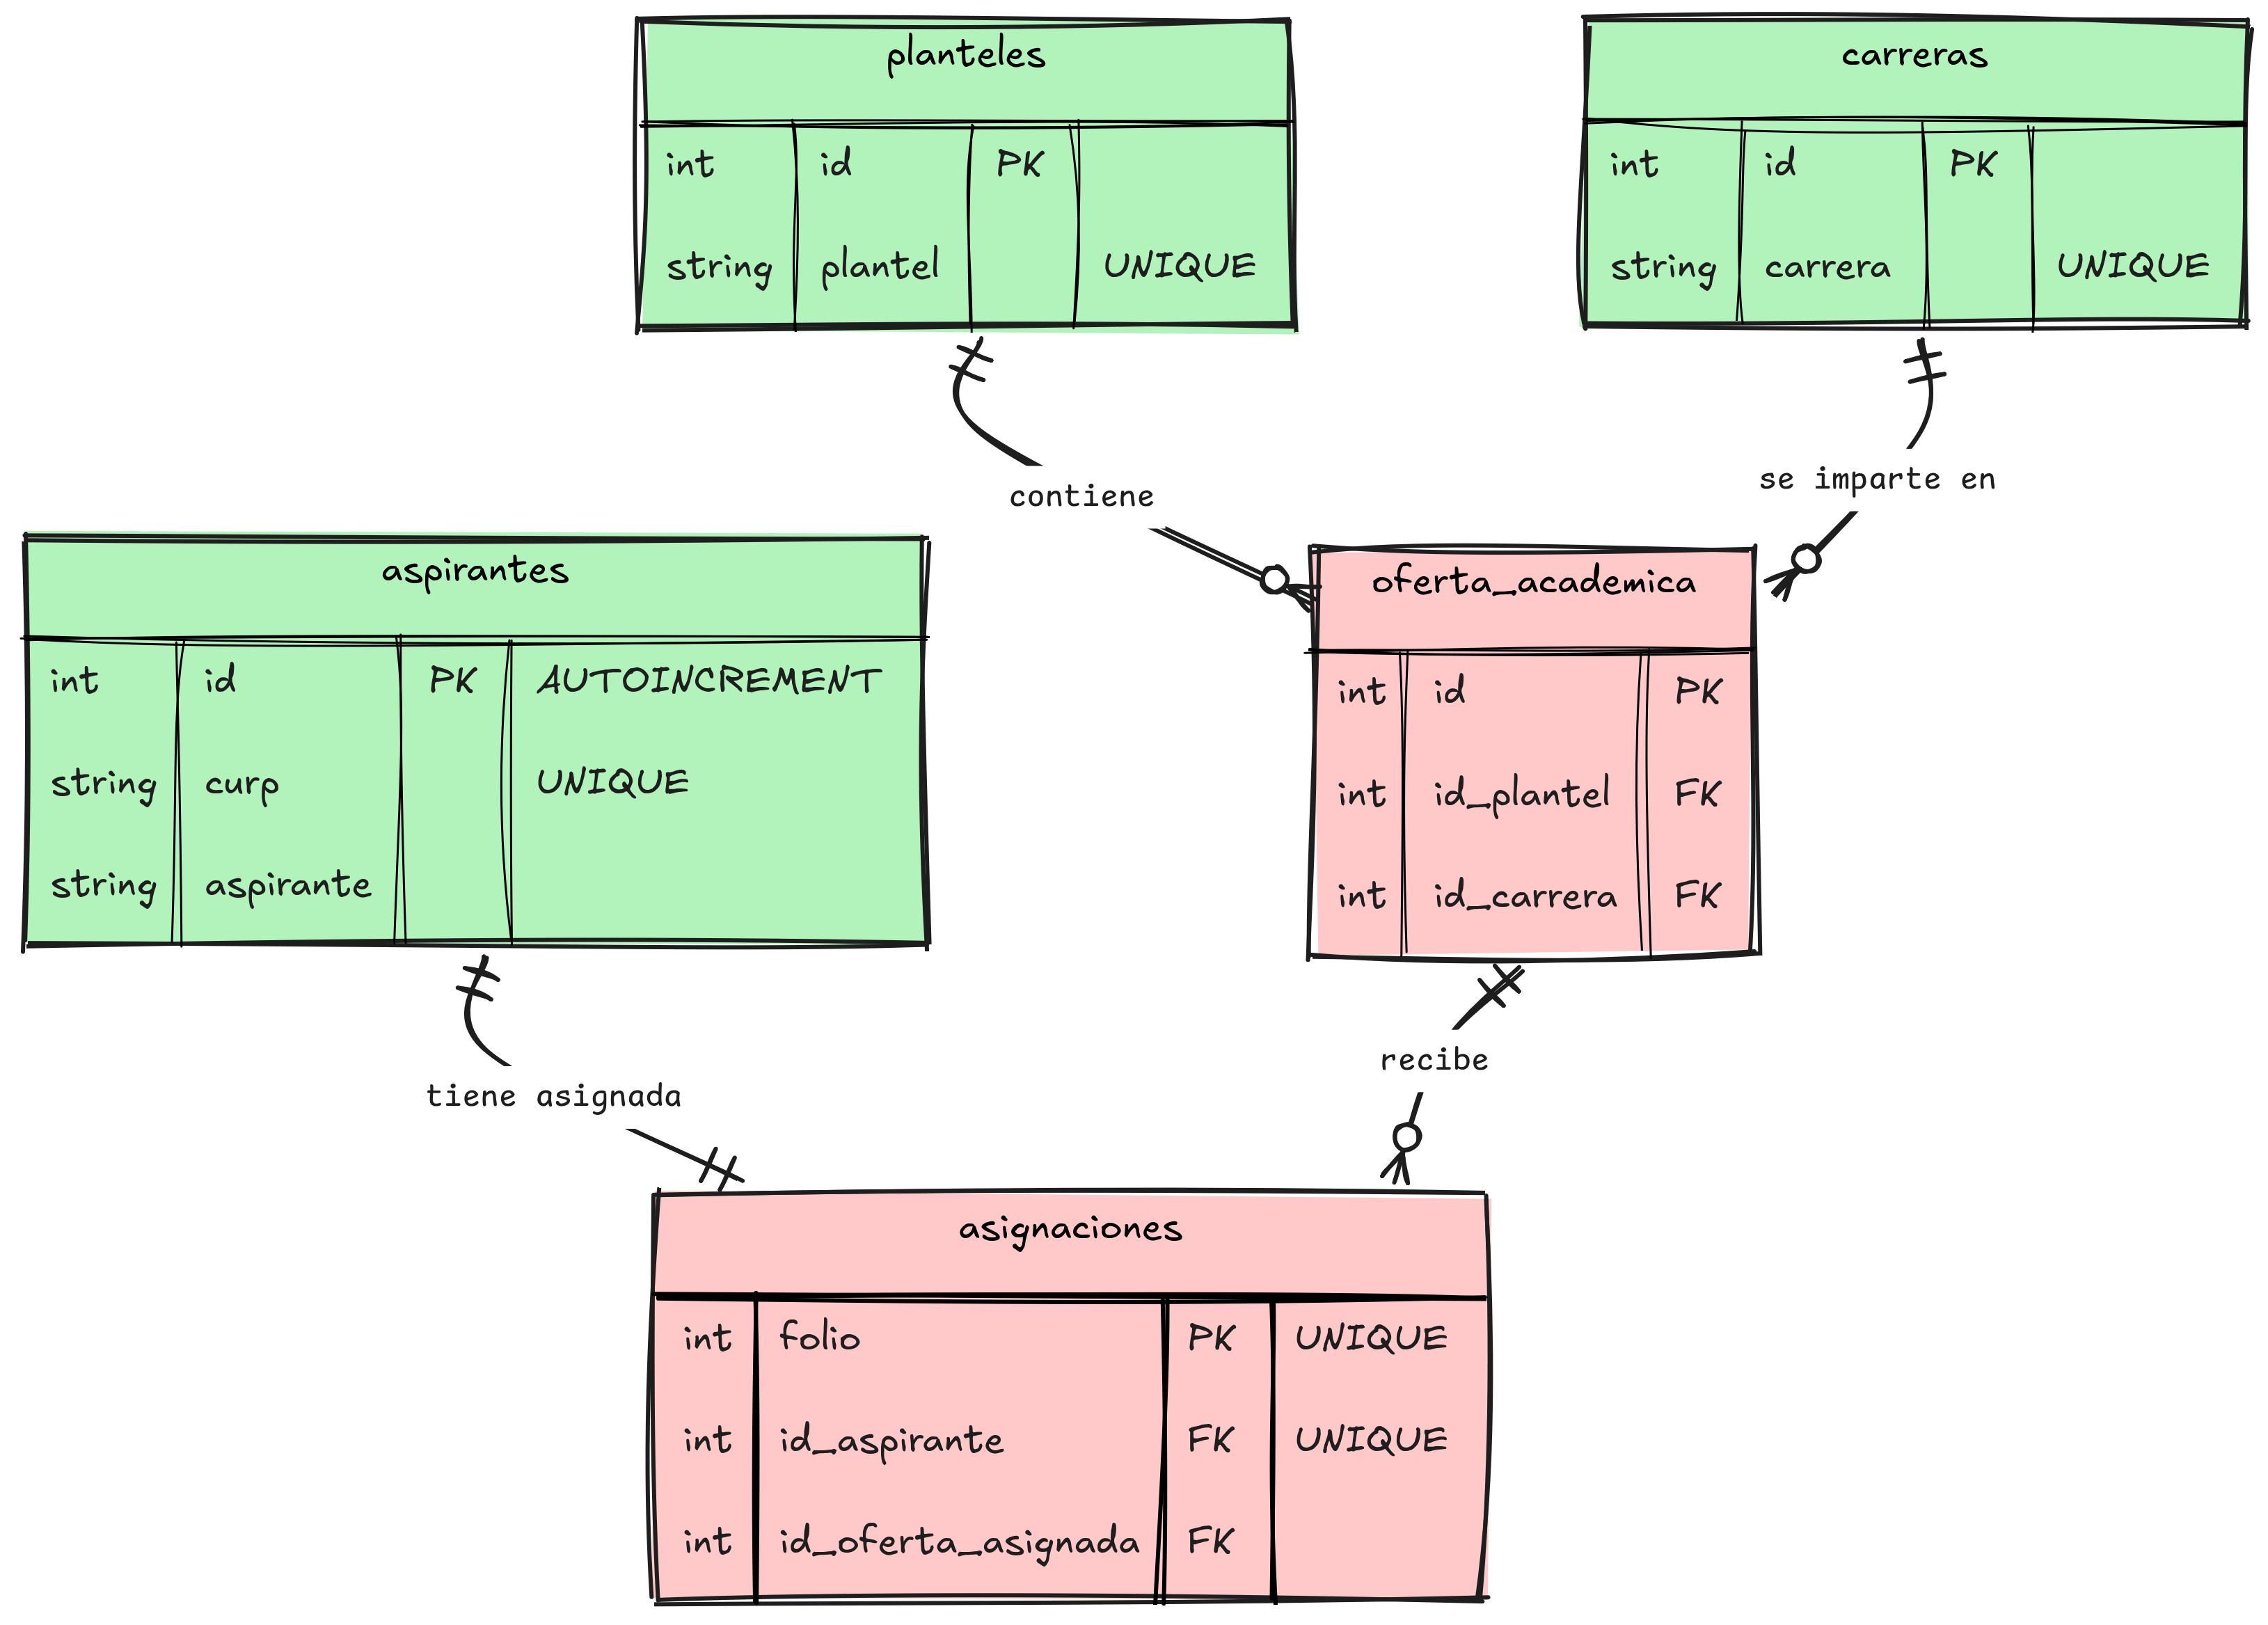
\includegraphics[width=0.95\textwidth]{./img/modelo-base-datos.png}
	\caption{Modelo de la base de datos}
	\label{fig:modelo-base-datos}
\end{figure}

% Tomando como base el punto anterior, redacta cada uno de los siguientes puntos:
%- Documenta y explica, las entidades que puedas identificar de tu base de datos, dibuja un diagrama donde las representes, que se muestren los nombres de las entidades y los campos de cada una, y abajo descríbelas.
% - Describe los tipos de relaciones que identifiques entre las entidades de tu base de datos.
% - Representa en forma tabular cada una de las entidades, es decir, en formato de tabla y llena cada una con al menos dos registros de ejemplo, datos ficticios.
% - Investiga y escribe las instrucciones de tipo lenguaje de definición de datos (LDD) y lenguaje de manipulación de datos (LMD) que podrían usarse para: crear una tabla (la que elijas) y otra para hacer una inserción y consulta de un registro en las tablas de la base de datos.
\subsection*{Entidades de la base de datos}
\addcontentsline{toc}{subsection}{Entidades de la base de datos}

Como se puede apreciar en la \textbf{Figura \ref{fig:modelo-base-datos}} y en la \textbf{Figura \ref{fig:modelo-bd-entidades}} se destacan cinco entidades para el modelado de los datos y se realiza un breve detallado de ellas. De forma adicional, consideramos las representaciones de los aspirantes, planteles y carreras técnicas como \textbf{entidades fuertes}, y por el otro lado, las representaciones de oferta académica y asignaciones como \textbf{entidades débiles}.

\begin{figure}[htb]
	\centering
	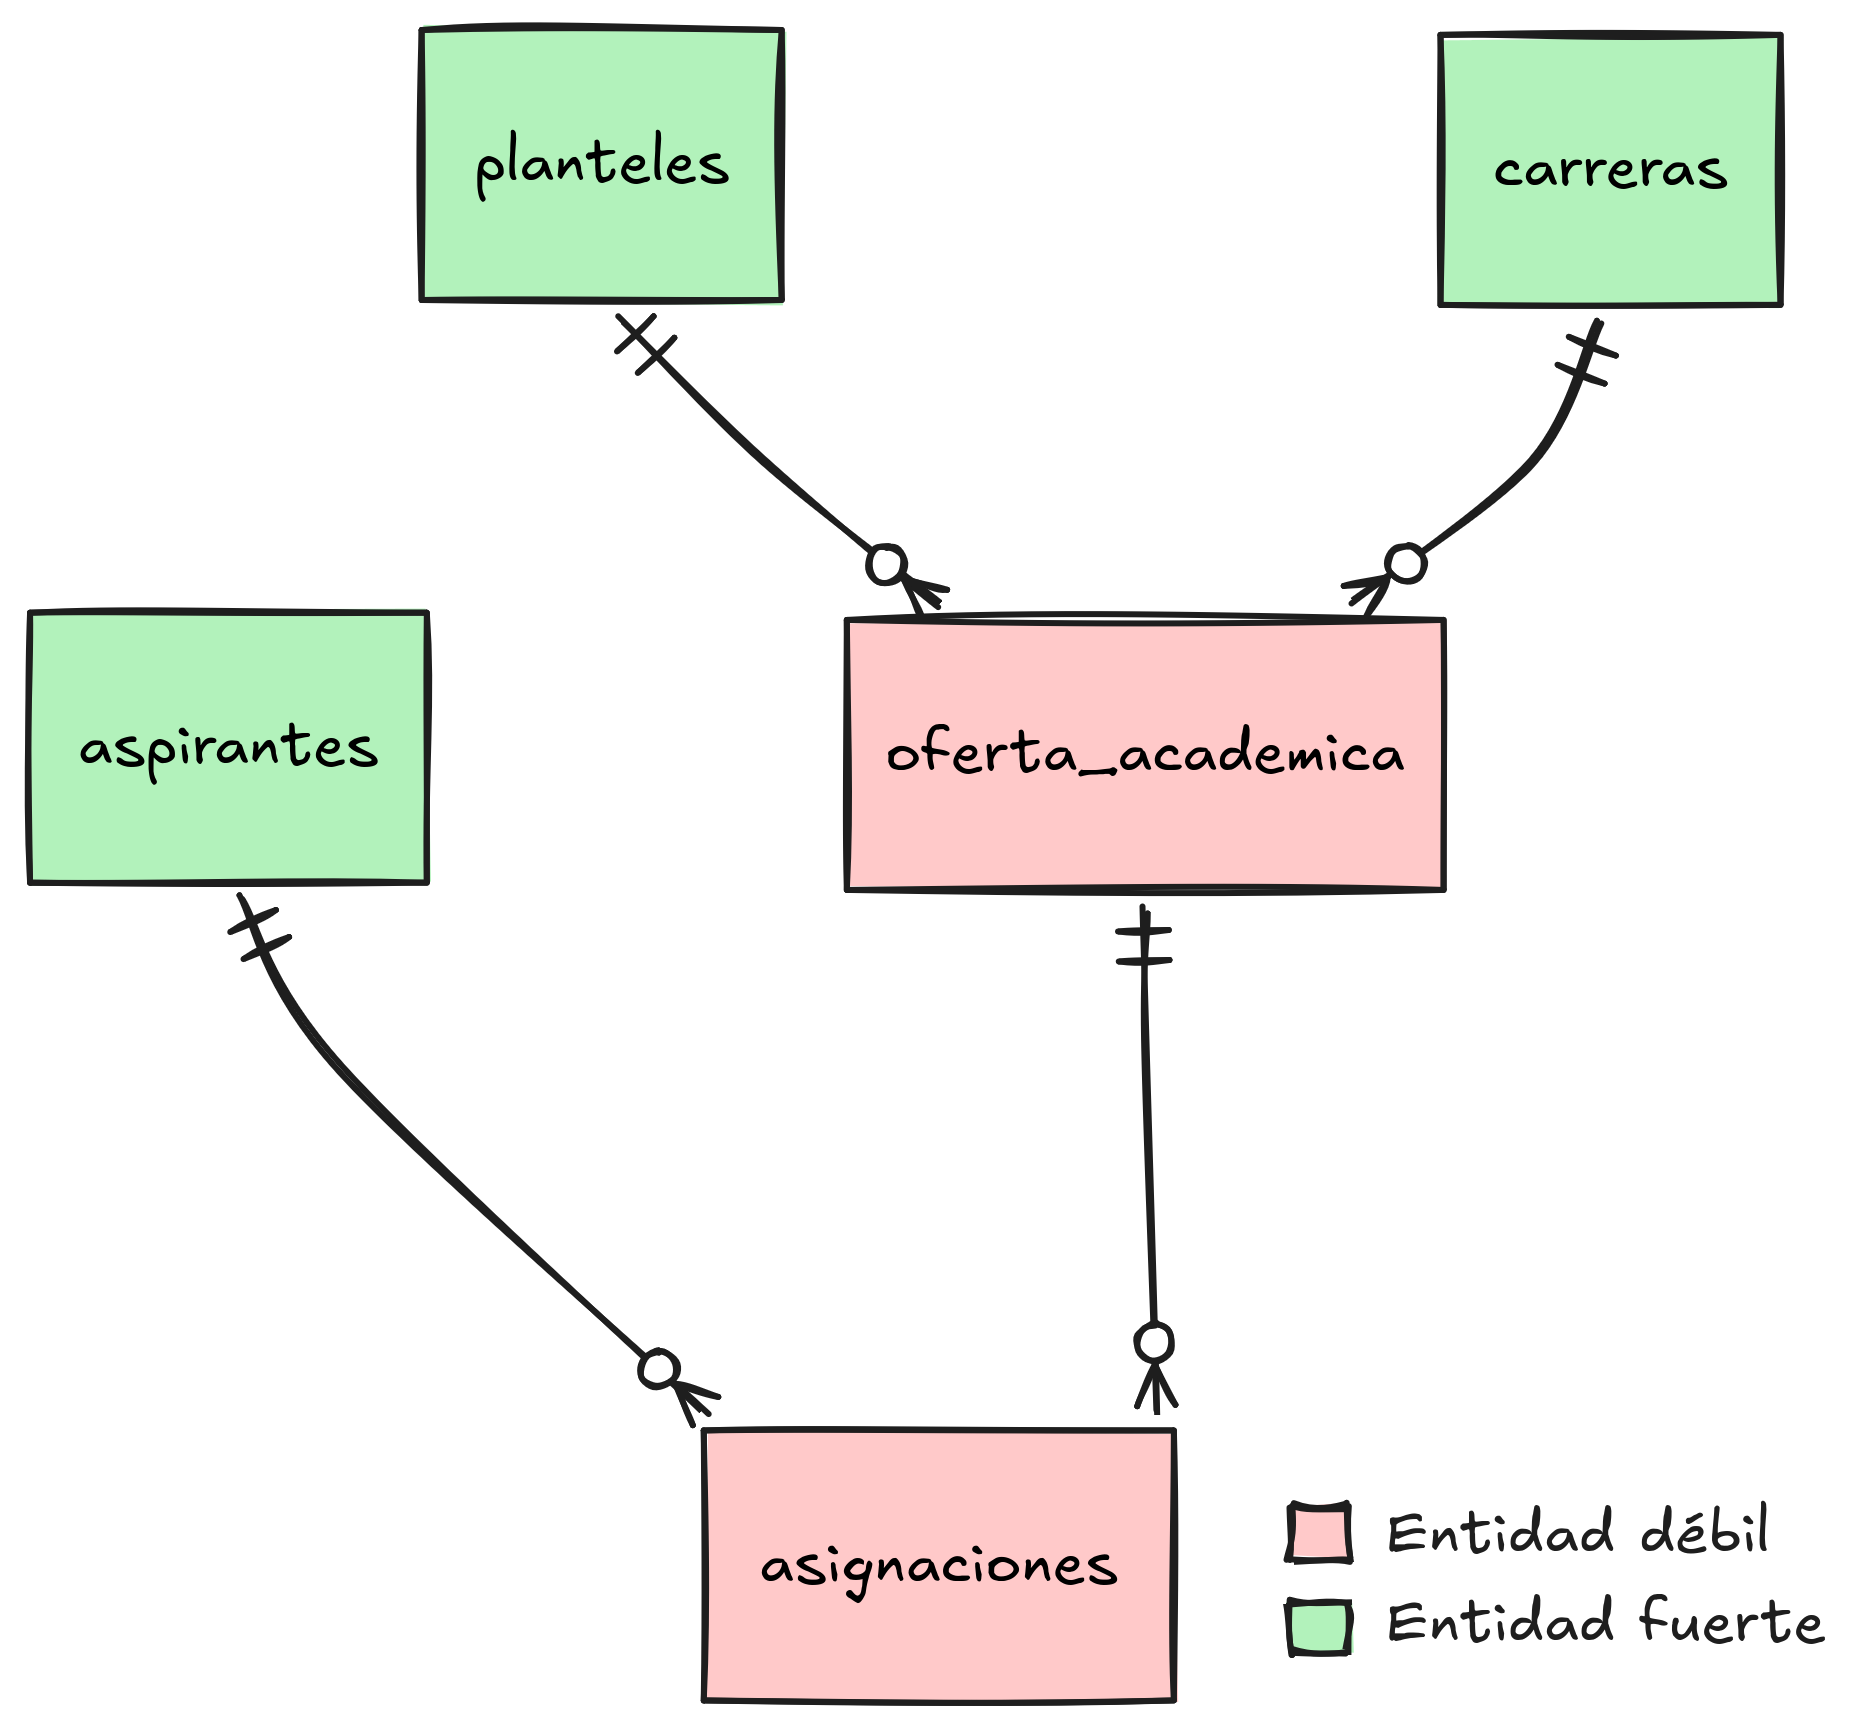
\includegraphics[width=0.6\textwidth]{./img/modelo-bd-entidades.png}
	\caption{Entidades de la base de datos}
	\label{fig:modelo-bd-entidades}
\end{figure}

\begin{itemize}
	\item \textbf{Asignaciones.} La entidad \texttt{asignaciones} representa las asignaciones de los aspirantes (egresados de la escuela secundaria) a un colegio de bachillerato técnico y el plantel y carrera técnica al que fue asignada el estudiante, decisión tomado por la autoridad competente en los criterios que haya dado a conocer en su momento. La entidad de las asignaciones tiene los siguientes campos:
		\begin{itemize}
			\item \textit{Identificador del aspirante.} El campo \texttt{id\_aspirante} permite identificar a un aspirante mediante un código númerico generado en el sistema de la institución en particular. El identificador es único; y este campo es una \textbf{llave foránea} que vincula el campo \texttt{id} de la entidad \texttt{aspirantes} con la entidad \texttt{asignaciones}.
			\item \textit{Oferta asignada.} El campo \texttt{id\_oferta\_asignada} permite identificar rápidamente la oferta académica que le corresponde al futuro alumno de media superior. Este campo es una llave \textbf{llave foránea} y hace referencia al campo \texttt{id} de la entidad \texttt{oferta\_academica}.
			\item \textit{Folio.} Un identificador único por asignación. La asignación es la oferta académica que estudiará el aspirante. La asignación es única por alumno. Además es una \textbf{llave primaria}.
		\end{itemize}
	\item \textbf{Aspirantes.} La entidad \texttt{aspirantes} representa a los alumnos egresados de secundaria, aspirantes al siguiente nivel educativo, y guarda algunos datos para la identicación del alumnado:
		\begin{itemize}
			\item \textit{CURP.} El campo \texttt{curp} almacena la clave CURP del alumno y [obviamente] es único. 
			\item \textit{Aspirante.} El campo \texttt{aspirante} guarda el nombre y apellido del aspirante. 
			\item \textit{Identificador de registro.} El campo \texttt{id} es una identicación única de la relación CURP-alumno; este campo está asignado como \textbf{llave primaria}.
		\end{itemize}
	\item \textbf{Oferta académica.} La entidad \texttt{oferta\_academica} son las carreras técnicas que ofrece cada uno de los planteles del bachillerato. Se almacena lo siguiente:
		\begin{itemize}
			\item \textit{Plantel.} El campo \texttt{id\_plantel} es una \textbf{llave foránea} que hace referencia al campo \texttt{id} de la entidad \texttt{planteles}. Representa los planteles que tienen abierta convocatoria para nuevo ingreso.
			\item \textit{Carrera.} El campo \texttt{id\_carrera} es una \textbf{llave foránea} que hace referencia al campo \texttt{id} de la entidad \texttt{carreras}. Representa las carreras que ofrece cada uno de los planteles.
			\item \textit{Identificador.} El campo \texttt{id} es la identicación única de cada oferta de carrera técnica ofrecida por un plantel. 
		\end{itemize}
	\item \textbf{Carreras.} La entidad \texttt{carreras} representa todas las carreras ofrecidas por la institución de bachillerato técnico.
		\begin{itemize}
			\item \textit{Identificador.} El campo \texttt{id} es una \textbf{llave primaria} que identifica vía númerica a un plantel.
			\item \textit{Plantel.} El campo \texttt{plantel} representa el nombre de un plantel conformado por el número del plantel y su ubicación; además cada nombre es único. 
		\end{itemize}
	\item \textbf{Planteles.} La entidad \texttt{planteles} representa todos los planteles de la institución academica.
		\begin{itemize}
			\item \textit{Identificador.} El campo \texttt{id} es una \textbf{llave primaria} que identifica de forma númerica una carrera técnica.
			\item \textit{Carrera.} Este campo (\texttt{carrera}) representa cada una de las carreras impartidas por la institución.
		\end{itemize}
\end{itemize}

\subsection*{Relaciones de la base de datos}
\addcontentsline{toc}{subsection}{Relaciones de la base de datos}

En la \textbf{ Figura \ref{fig:relaciones-entidades}} y en el \textbf{Cuadro \ref{tab:tipos-relaciones}} se visualizan las relaciones entre las entidades y su cardinalidad.

\begin{figure}[htb]
	\centering
	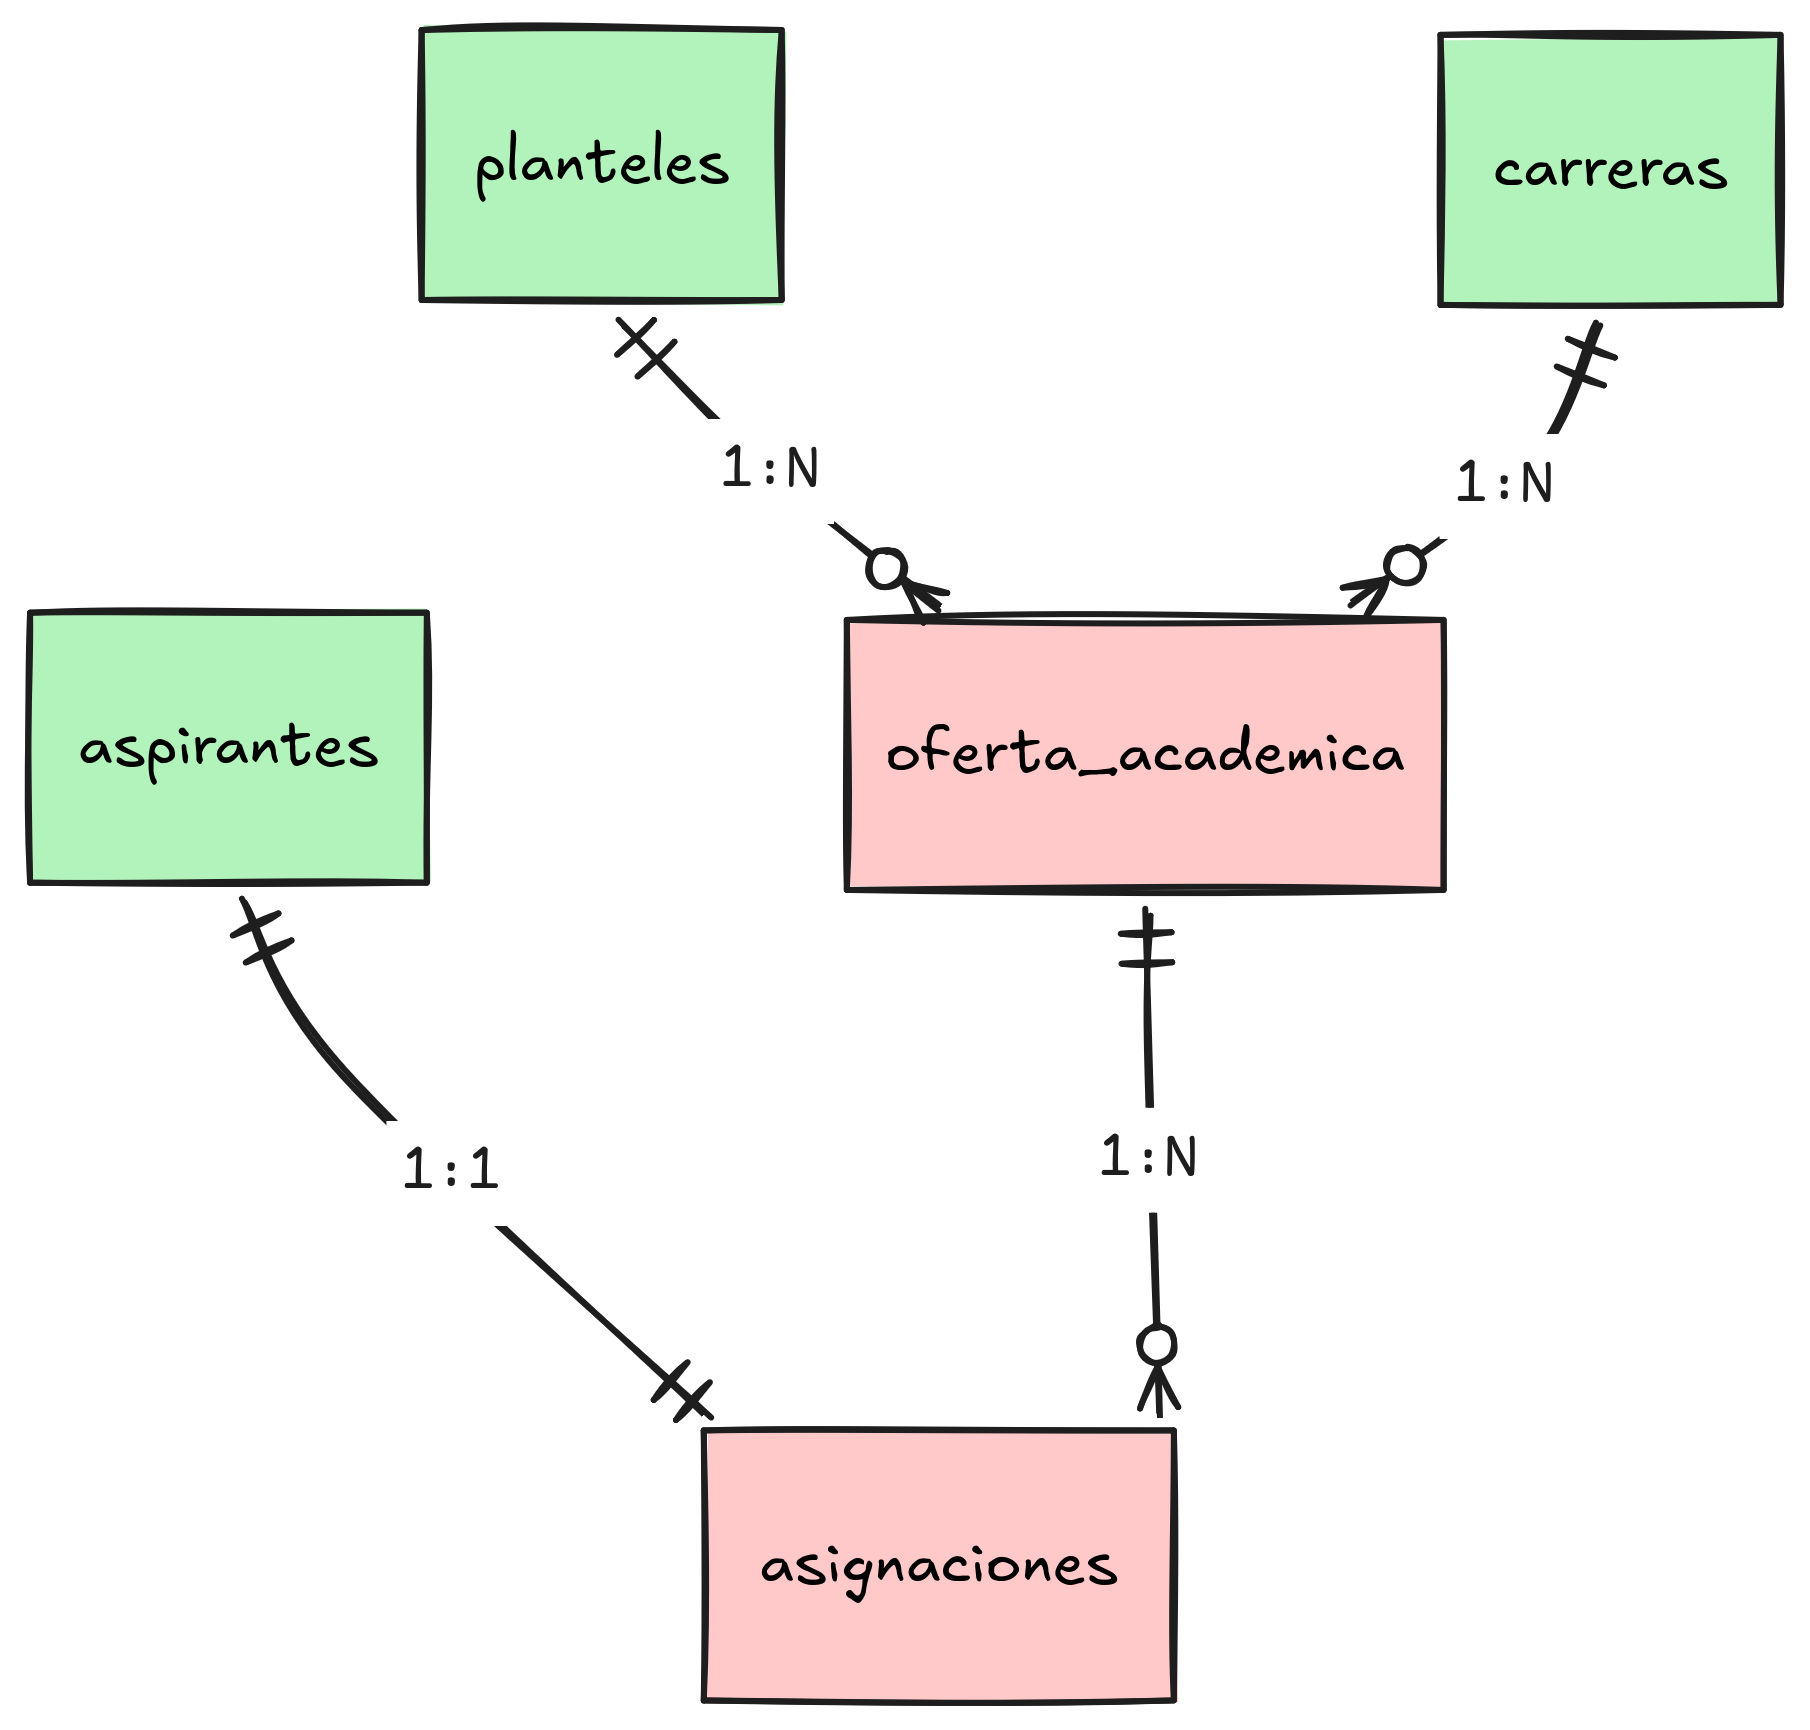
\includegraphics[width=0.5\textwidth]{./img/relaciones-entidades.png}
	\caption{Relaciones entre entidades}
	\label{fig:relaciones-entidades}
\end{figure}

\begin{table}[h!]
	\begin{center}
		\begin{tabular}{l|l|p{5cm}}
			\hline
			\textbf{Relación} & \textbf{Tipo} & \textbf{Descripción} \\
			\hline
			\texttt{aspirantes} $\longmapsto$ \texttt{asignaciones} & 1:1 & Un aspirante solo puede tener un oferta asignada y las ofertas asignadas son únicas. \\
			\hline
			\texttt{oferta\_academica} $\longmapsto$ \texttt{asignaciones} & 1:N & Una oferta academica puede estar asignado a varios aspirantes, y todas las asignaciones vincula una única oferta. \\
			\hline
			\texttt{planteles} $\longmapsto$ \texttt{oferta\_academica} & 1:N & Un plantel puede ofrecer una variedad de ofertas, pero cada oferta es única. \\
			\hline
			\texttt{carreras} $\longmapsto$ \texttt{oferta\_academica} & 1:N & Una carrera técnica puede ser impartida por muchos planteles, pero la impartición de la carrera es única. \\
			\hline
		\end{tabular}
		\caption{Tipos de relaciones}
		\label{tab:tipos-relaciones}
	\end{center}
\end{table}

\subsection*{Representación tabular de las entidades}
\addcontentsline{toc}{subsection}{Representación tabular de las entidades}

A continuación se presenta las entidades mediante la tabulación y se muestra datos ficticios para facilitar la interpretación. En los \textbf{Cuadros \ref{tab:asignaciones}, \ref{tab:aspirantes}, \ref{tab:oferta-academica}, \ref{tab:planteles}} y \textbf{\ref{tab:carreras}}.

\begin{table}[h!]
	\begin{center}
		\begin{tabular}{p{4cm}|p{4cm}|p{6.51cm}}
			\hline
			\textbf{\texttt{folio}} & \textbf{\texttt{id\_aspirante}} & \textbf{\texttt{id\_oferta\_academica}} \\
			\hline
			\texttt{7957} & \texttt{7957123} & \texttt{1} \\
			\texttt{4843} & \texttt{4843123} & \texttt{2} \\
			\texttt{6967} & \texttt{6967123} & \texttt{3} \\
			\hline
		\end{tabular}
		\caption{Tabulación de \texttt{asignaciones}}
		\label{tab:asignaciones}
	\end{center}
\end{table}

\begin{table}[h!]
	\begin{center}
		\begin{tabular}{p{3cm}|p{4.836666667cm}|l}
			\hline
			\textbf{\texttt{id}} & \textbf{\texttt{curp}} & \textbf{\texttt{aspirante}} \\
			\hline
			\texttt{4843123} & \texttt{XEXX010101MNEXXXA8} & \texttt{Arreola Islas Johana Guadalupe} \\
			\texttt{6967123} & \texttt{XEXX010101HNEXXXA3} & \texttt{Benigno Loma Anahi} \\
			\texttt{7957123} & \texttt{XEXX010101HNEXXXA4} & \texttt{Antonio Ignacio Nahomi Jireth} \\
			\hline
		\end{tabular}
		\caption{Tabulación de \texttt{aspirantes}}
		\label{tab:aspirantes}
	\end{center}
\end{table}

\begin{table}[h!]
	\begin{center}
		\begin{tabular}{p{4cm}|p{4cm}|p{6.51cm}}
			\hline
			\textbf{\texttt{id}} & \textbf{\texttt{id\_plantel}} & \textbf{\texttt{id\_carrera}} \\
			\hline
			\texttt{1} & \texttt{1} & \texttt{1} \\
			\texttt{2} & \texttt{1} & \texttt{2} \\
			\texttt{3} & \texttt{2} & \texttt{1} \\
			\hline
		\end{tabular}
		\caption{Tabulación de \texttt{oferta\_academica}}
		\label{tab:oferta-academica}
	\end{center}
\end{table}

\begin{table}[h!]
	\begin{center}
		\begin{tabular}{p{7.255cm}|p{7.255cm}}
			\hline
			\textbf{\texttt{id}} & \textbf{\texttt{plantel}} \\
			\hline
			\texttt{1} & \texttt{Plantel Cancún I} \\
			\texttt{2} & \texttt{Plantel Cancún II} \\
			\hline
		\end{tabular}
		\caption{Tabulación de \texttt{planteles}}
		\label{tab:planteles}
	\end{center}
\end{table}

\begin{table}[h!]
	\begin{center}
		\begin{tabular}{p{7.255cm}|p{7.255cm}}
			\hline
			\textbf{\texttt{id}} & \textbf{\texttt{carrera}} \\
			\hline
			\texttt{1} & \texttt{Interpretación Mecanicista de IA} \\
			\texttt{2} & \texttt{Machine Unlearning} \\
			\hline
		\end{tabular}
		\caption{Tabulación de \texttt{carreras}}
		\label{tab:carreras}
	\end{center}
\end{table}

\subsection*{Instrucciones de LDD y LMD para la base de datos}
\addcontentsline{toc}{subsection}{Instrucciones de LDD y LMD para la base de datos}

Los esquemas de las bases de datos se especifican mediante un conjunto de definiciones expresadas mediante un lenguaje especial denominado \textbf{lenguaje de definición de datos} (LDD)~\cite{Silberschatz2014}. A continuación se muestra un ejemplo de instrucción LDD para la implementación de la base de datos anterior:

\lstinputlisting[language=SQL, caption=Instrucciones LDD]{./sql/ldd.sql}

Un lenguaje de manipulación de datos (LMD) es un lenguaje que permite a los usuarios tener acceso a los datos organizados mediante el modelo de datos correspondiente, o manipularlos~\cite{Silberschatz2014}. A continuación se muestra ejemplos de este tipo de instrucciones:

\lstinputlisting[language=SQL, caption=Instrucciones LMD]{./sql/lmd.sql}


% Investiga y presenta una imagen de un esquema de una base de datos no relacional, una base de datos orientada a objetos y una base de datos orientada a documentos. Da una breve descripción de lo que observas en cada uno de los esquemas que presentas. Considerando similitudes y diferencias, con base a sus definiciones y comparadas con las bases de datos relacionales.
\section*{Otros tipos de bases de datos}
\addcontentsline{toc}{section}{Otros tipos de base de datos}

\paragraph{Bases de datos no relacional}
Las bases de datos NoSQL~\cite{ibm} no son relacionales y elimina la necesidad de conectar tablas, por lo que sus capacidades de fragmentación y alta disponibilidad facilitan el escalado horizontal sin aumentar vertiginosamente la potencia de hardware. El escalado vertical es el aumento de las capacidades del hardware, mientras que el escalado horizontal es el aumento de la captación de tipos de datos e información. Un ejemplo de este tipo de bases de datos no relacional es el \textbf{almacén de valores clave}~\cite{ibm}, esto es lo que maneja gestores como \textit{Redis} y \textit{Memcached}. 

\paragraph{Bases de datos orientado a documentos}
Otro ejemplo es el \textbf{almacén de documentos}~\cite{ibm} como \textit{MongoDB}. En la \textbf{Figura \ref{fig:bd-json}} se presenta una visualización de una base de datos de documentos. En este estos documentos se almacena información sobre un objeto y cualquiera de sus metadatos relacionados, los documentos almacenan datos en pares de campo-valor y los formatos del documento pueden ser JSON, BSON, o XML~\cite{mongodb}.

\begin{figure}[h!]
	\centering
	\begin{subfigure}[b]{0.45\linewidth}
		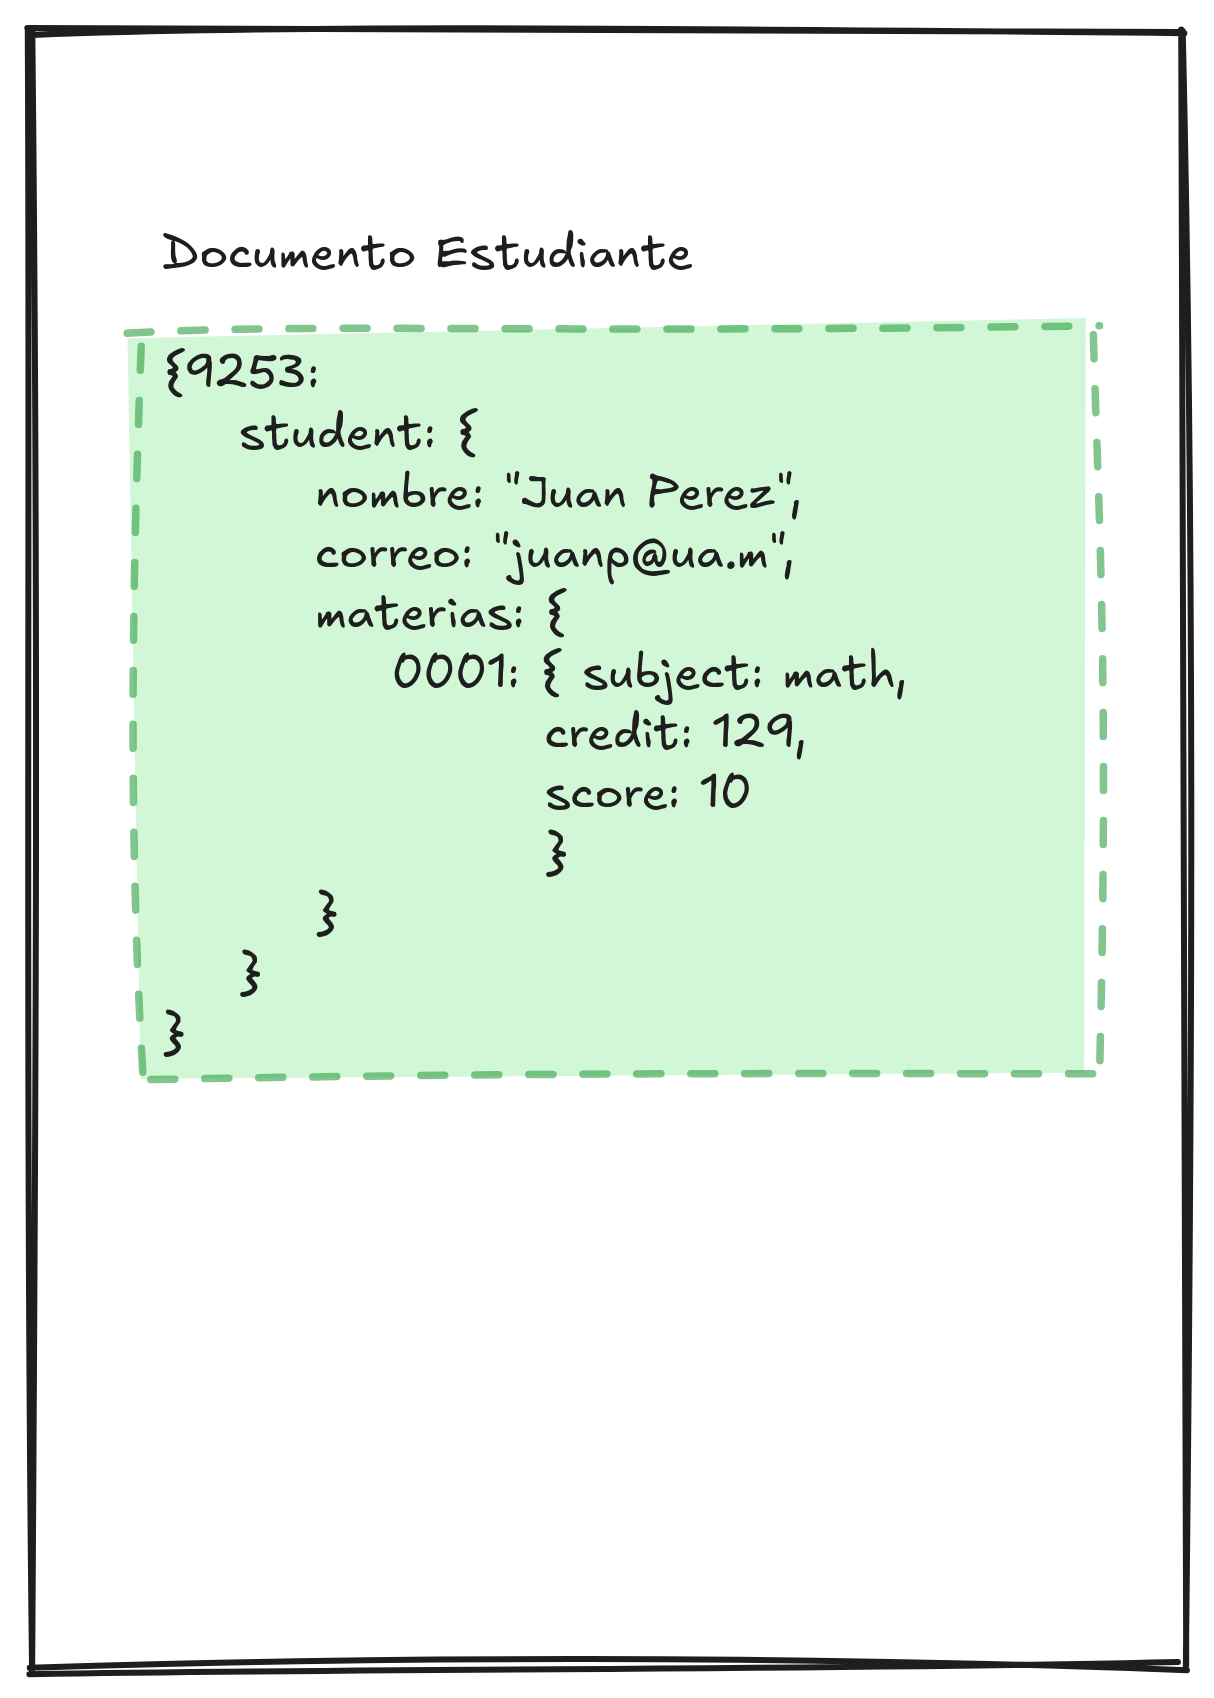
\includegraphics[width=\linewidth]{./img/bd-json.png}
		\caption{Orientado a documentos}
		\label{fig:bd-json}
	\end{subfigure}
	\begin{subfigure}[b]{0.295\linewidth}
		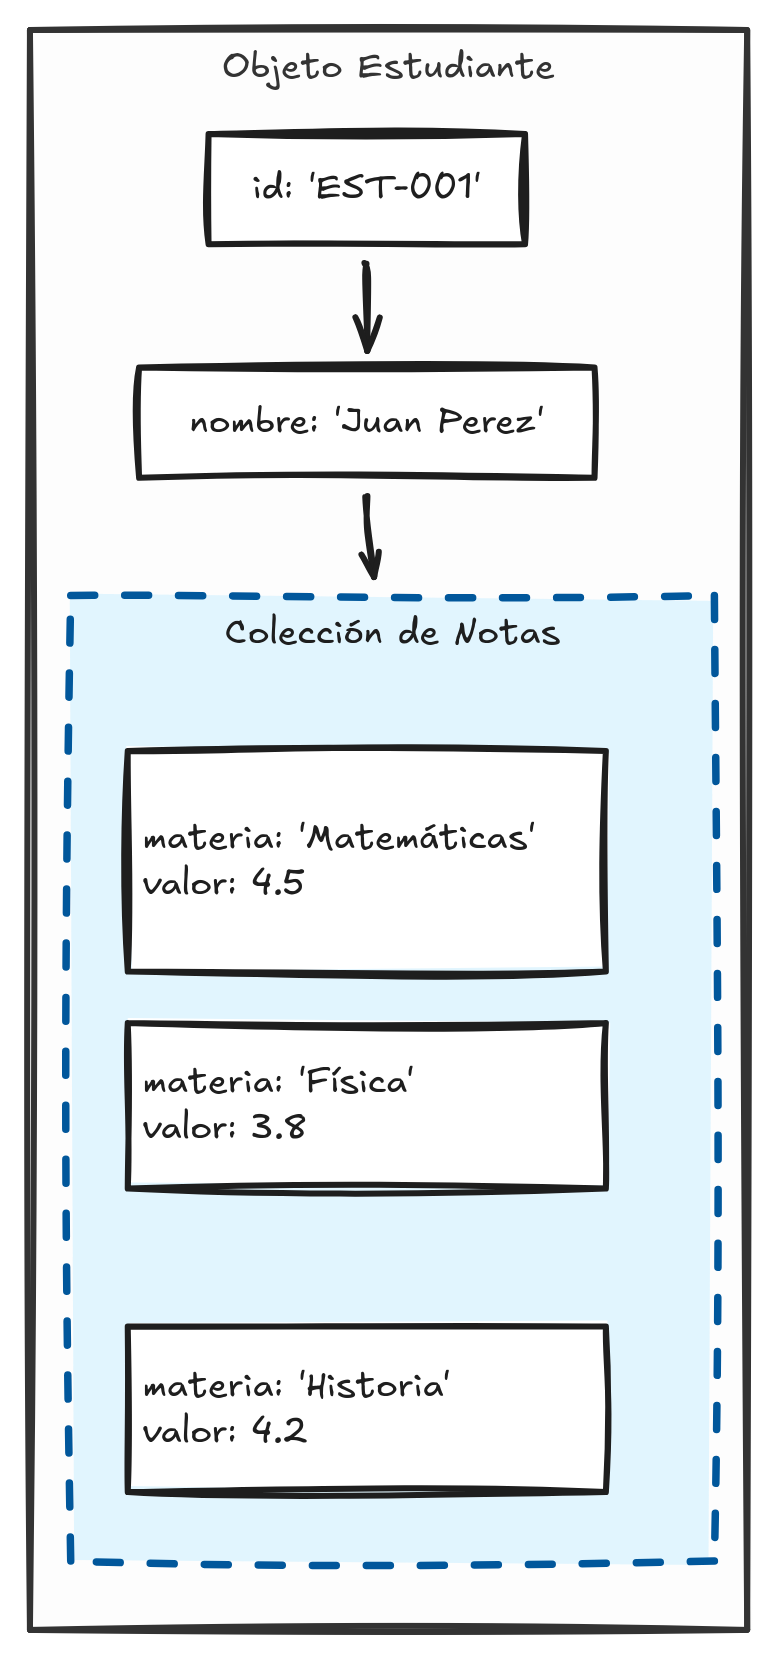
\includegraphics[width=\linewidth]{./img/bd-objetos.png}
		\caption{Orientado a objetos}
		\label{fig:bd-objeto}
	\end{subfigure}
	\caption{Base de datos no relacionales}
	\label{fig:base-nosql}
\end{figure}

\paragraph{Base de datos orientada a objetos}
Las bases de datos orientadas a objetos representan el mundo real y resuelve problemas a través de objetos (tangibles o digitales)~\cite{unam}. En la \textbf{Figura \ref{fig:bd-objeto}} se muestra un ejemplo de este tipo de bases de datos.

La similitud entre las bases de datos orientado a objetos y a documentos es que no están bajo el formato de tabla como representación de datos. La principal diferencia es que las bases de datos orientado a objetos se realizan con una implementación abstracta similar a la programación orientada a objetos (OOP), mientras que la base de datos orientada a documentos hace uso de estructuras como JSON o XML, donde la capacidad de extensión de campos y metadatos se pueden hacer de forma rápida y sencilla sin romper la relación con los archivos existentes y posteriores. Para realizar el escalado de campos o metadatos en una base de datos orientado a objeto se requiere aplicar conceptos de herencia y otras complejidades al estilo de la OOP; y brinda un desarrollo de la base de datos muy lento al principio y a medida que pasa la fase inicial, el mantenimiento es relativamente sencilla.

% Escribe una conclusión de media cuartilla aproximadamente, respondiendo a preguntas como:
%¿Cuáles son las ventajas de las bases de datos relacionales?
%¿Qué desventajas tienen frente a otros modelos?
%¿En qué contextos serían más adecuadas las bases de datos no relacionales?
\section*{Conclusión}
\addcontentsline{toc}{section}{Conclusión}

Las bases de datos relacionales son el tipo de bases de datos más usadas por la relativa sencillez y practicidad de su modelado de datos basado en tablas y relaciones de ellas, sin embargo, a medida que se requiere aumentar el volumen de datos o la captación de campos o metadatos se requiere aumentar la capacidad computacional y la complejidad de relacionar los datos existentes aumenta de forma considerable. Esto no sucede si se emplea bases de datos relacionales que ayudan al aumento de la captación de campos de datos o metadatos sin requerir aumento de capacidad computacional. Sin embargo, la visualización de datos en las llamadas bases de datos relacionales son complicados de representar de manera amigable para aquellos no son técnicos cuando se requiere conocer múltiples fuentes de información, algo que las bases de datos relacionales solucionan presentando al usuario una tabla modificada. Las bases de datos no relacionales son útiles para la web y sistemas de caché, pero para la mayoría de los usos informáticos una base de datos relacional funciona y es más fácil de implementar.

\newpage

% ========== Bibliografía =======
%\nocite{*}
\printbibliography[heading=bibintoc, title={Referencias}]
\newpage

\listoftables
\listoffigures
\lstlistoflistings
\newpage

\end{document}